\chapter{問題定義與方法}
\label{c:method}

\section{目標與啟發}

本研究最終目標是希望能改善對車內人臉的偵測結果,因此首先我們先觀察為何一般人臉偵測做在車內人臉上無法獲得我們期望的結果。透過觀察幾個較常見的人臉資料集,如 Wider Face~\cite{yang2016wider} 和 AFW~\cite{zhu2012face} 等,我們發現資料集中大部分都是在正常光照下的圖片 (如圖~\ref{fig:general_fac})。而與之相比,車內影像受到車輛移動的影響,會暴露於各種不同的光照下 (如圖~\ref{fig:incar_face}),使測試資料的光照更加多元而難以偵測出人臉。

\begin{figure}[t]
\centering
\begin{subfigure}[b]{0.3\textwidth}
    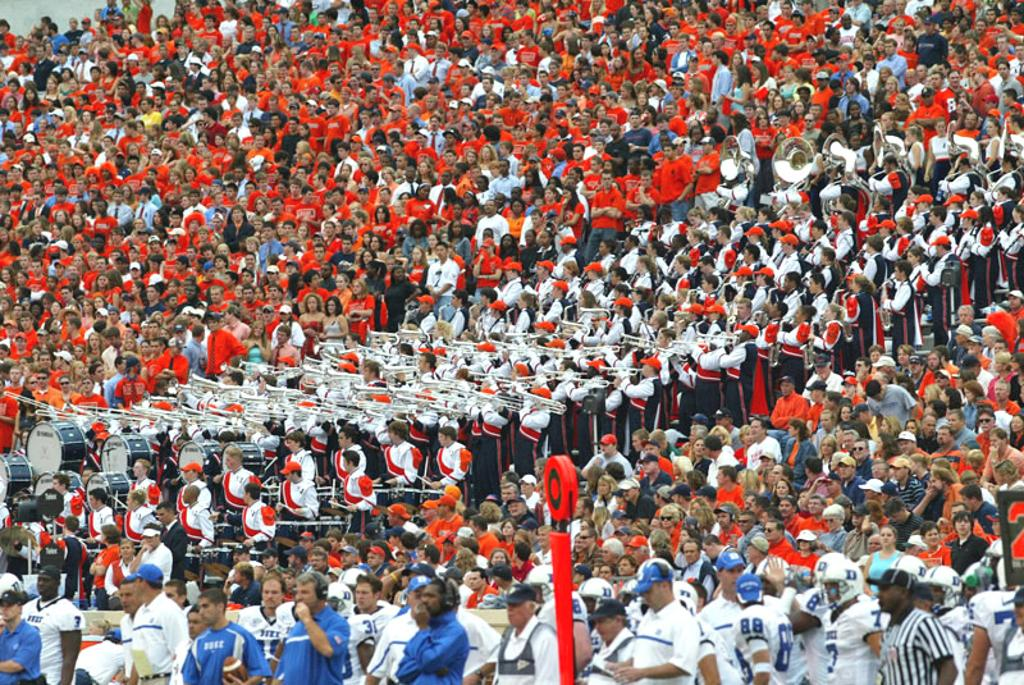
\includegraphics[width=\textwidth]{figures/data_1}
\end{subfigure}
\begin{subfigure}[b]{0.3\textwidth}
    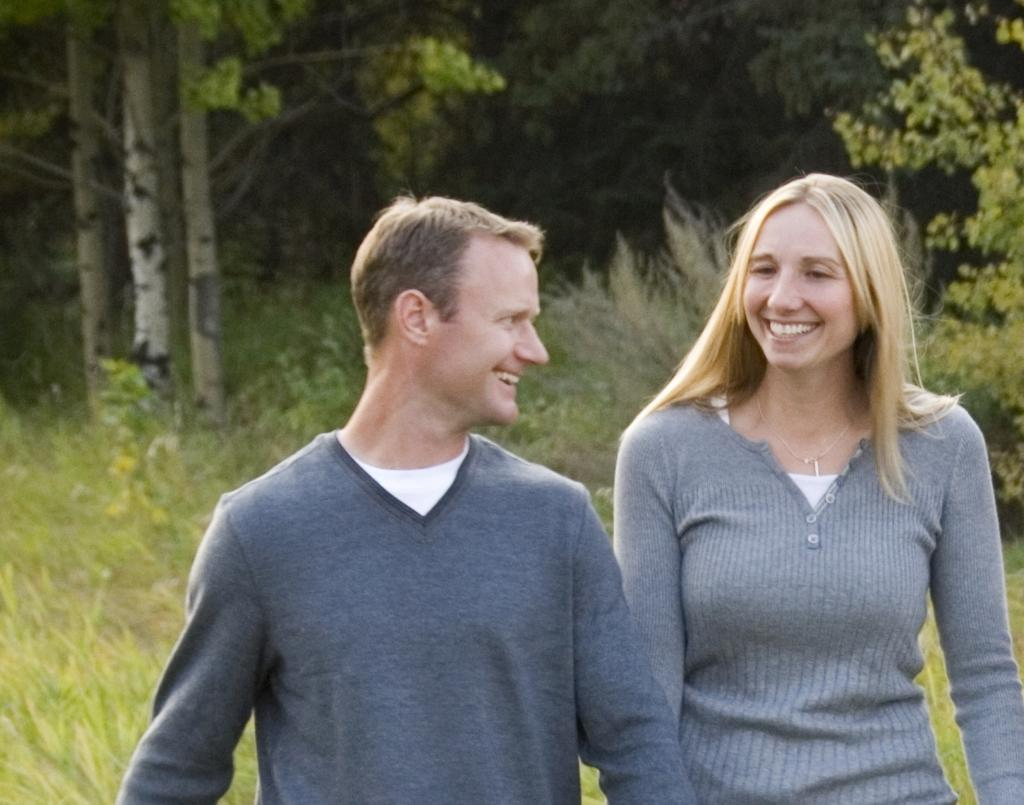
\includegraphics[width=\textwidth]{figures/data_2}
\end{subfigure}
\begin{subfigure}[b]{0.3\textwidth}
    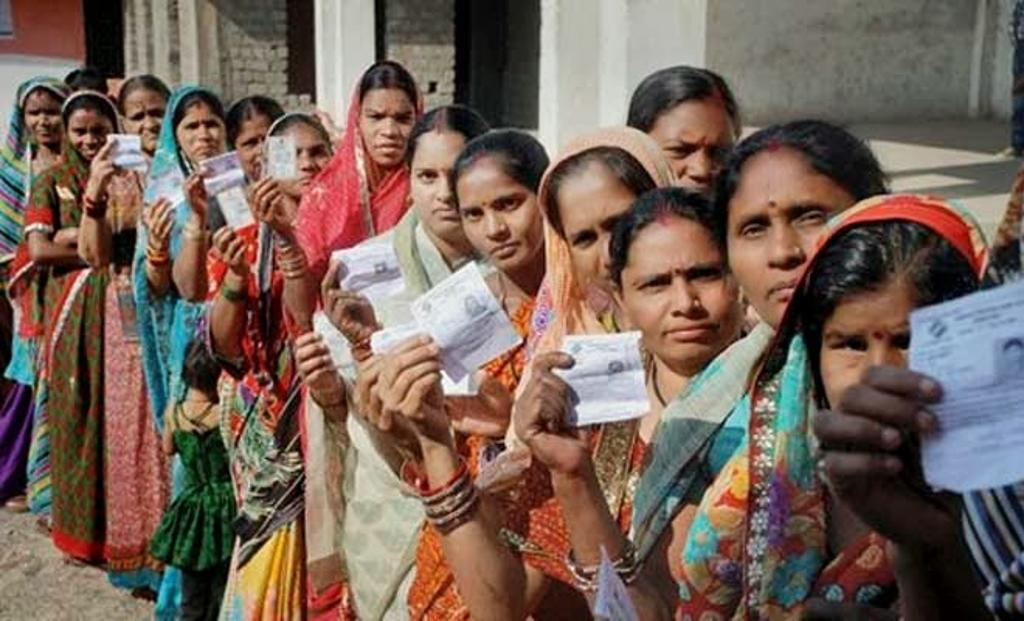
\includegraphics[width=\textwidth]{figures/data_3}
\end{subfigure}
\begin{subfigure}[b]{0.3\textwidth}
    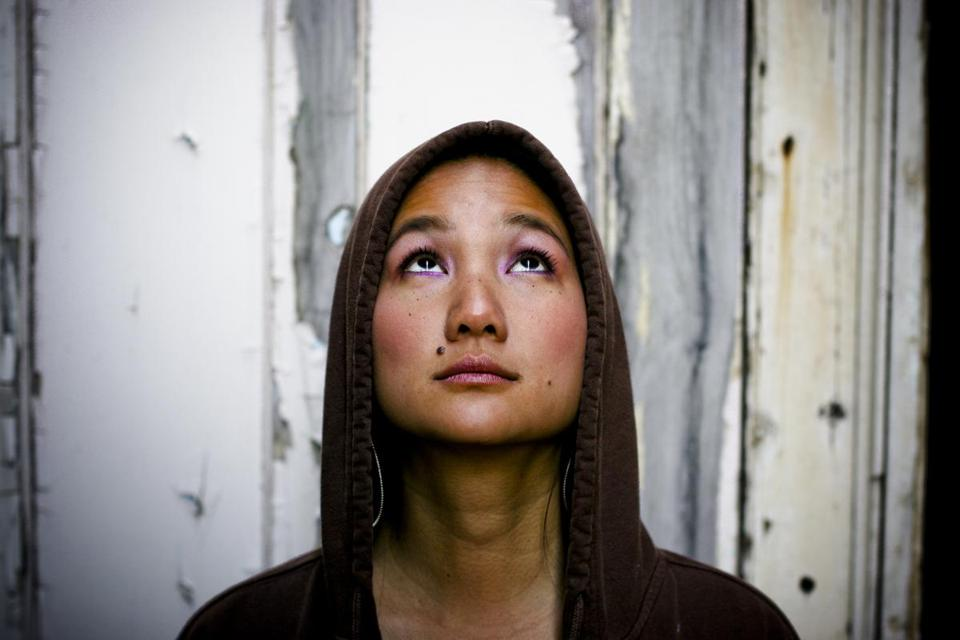
\includegraphics[width=\textwidth]{figures/data_4}
\end{subfigure}
\begin{subfigure}[b]{0.3\textwidth}
    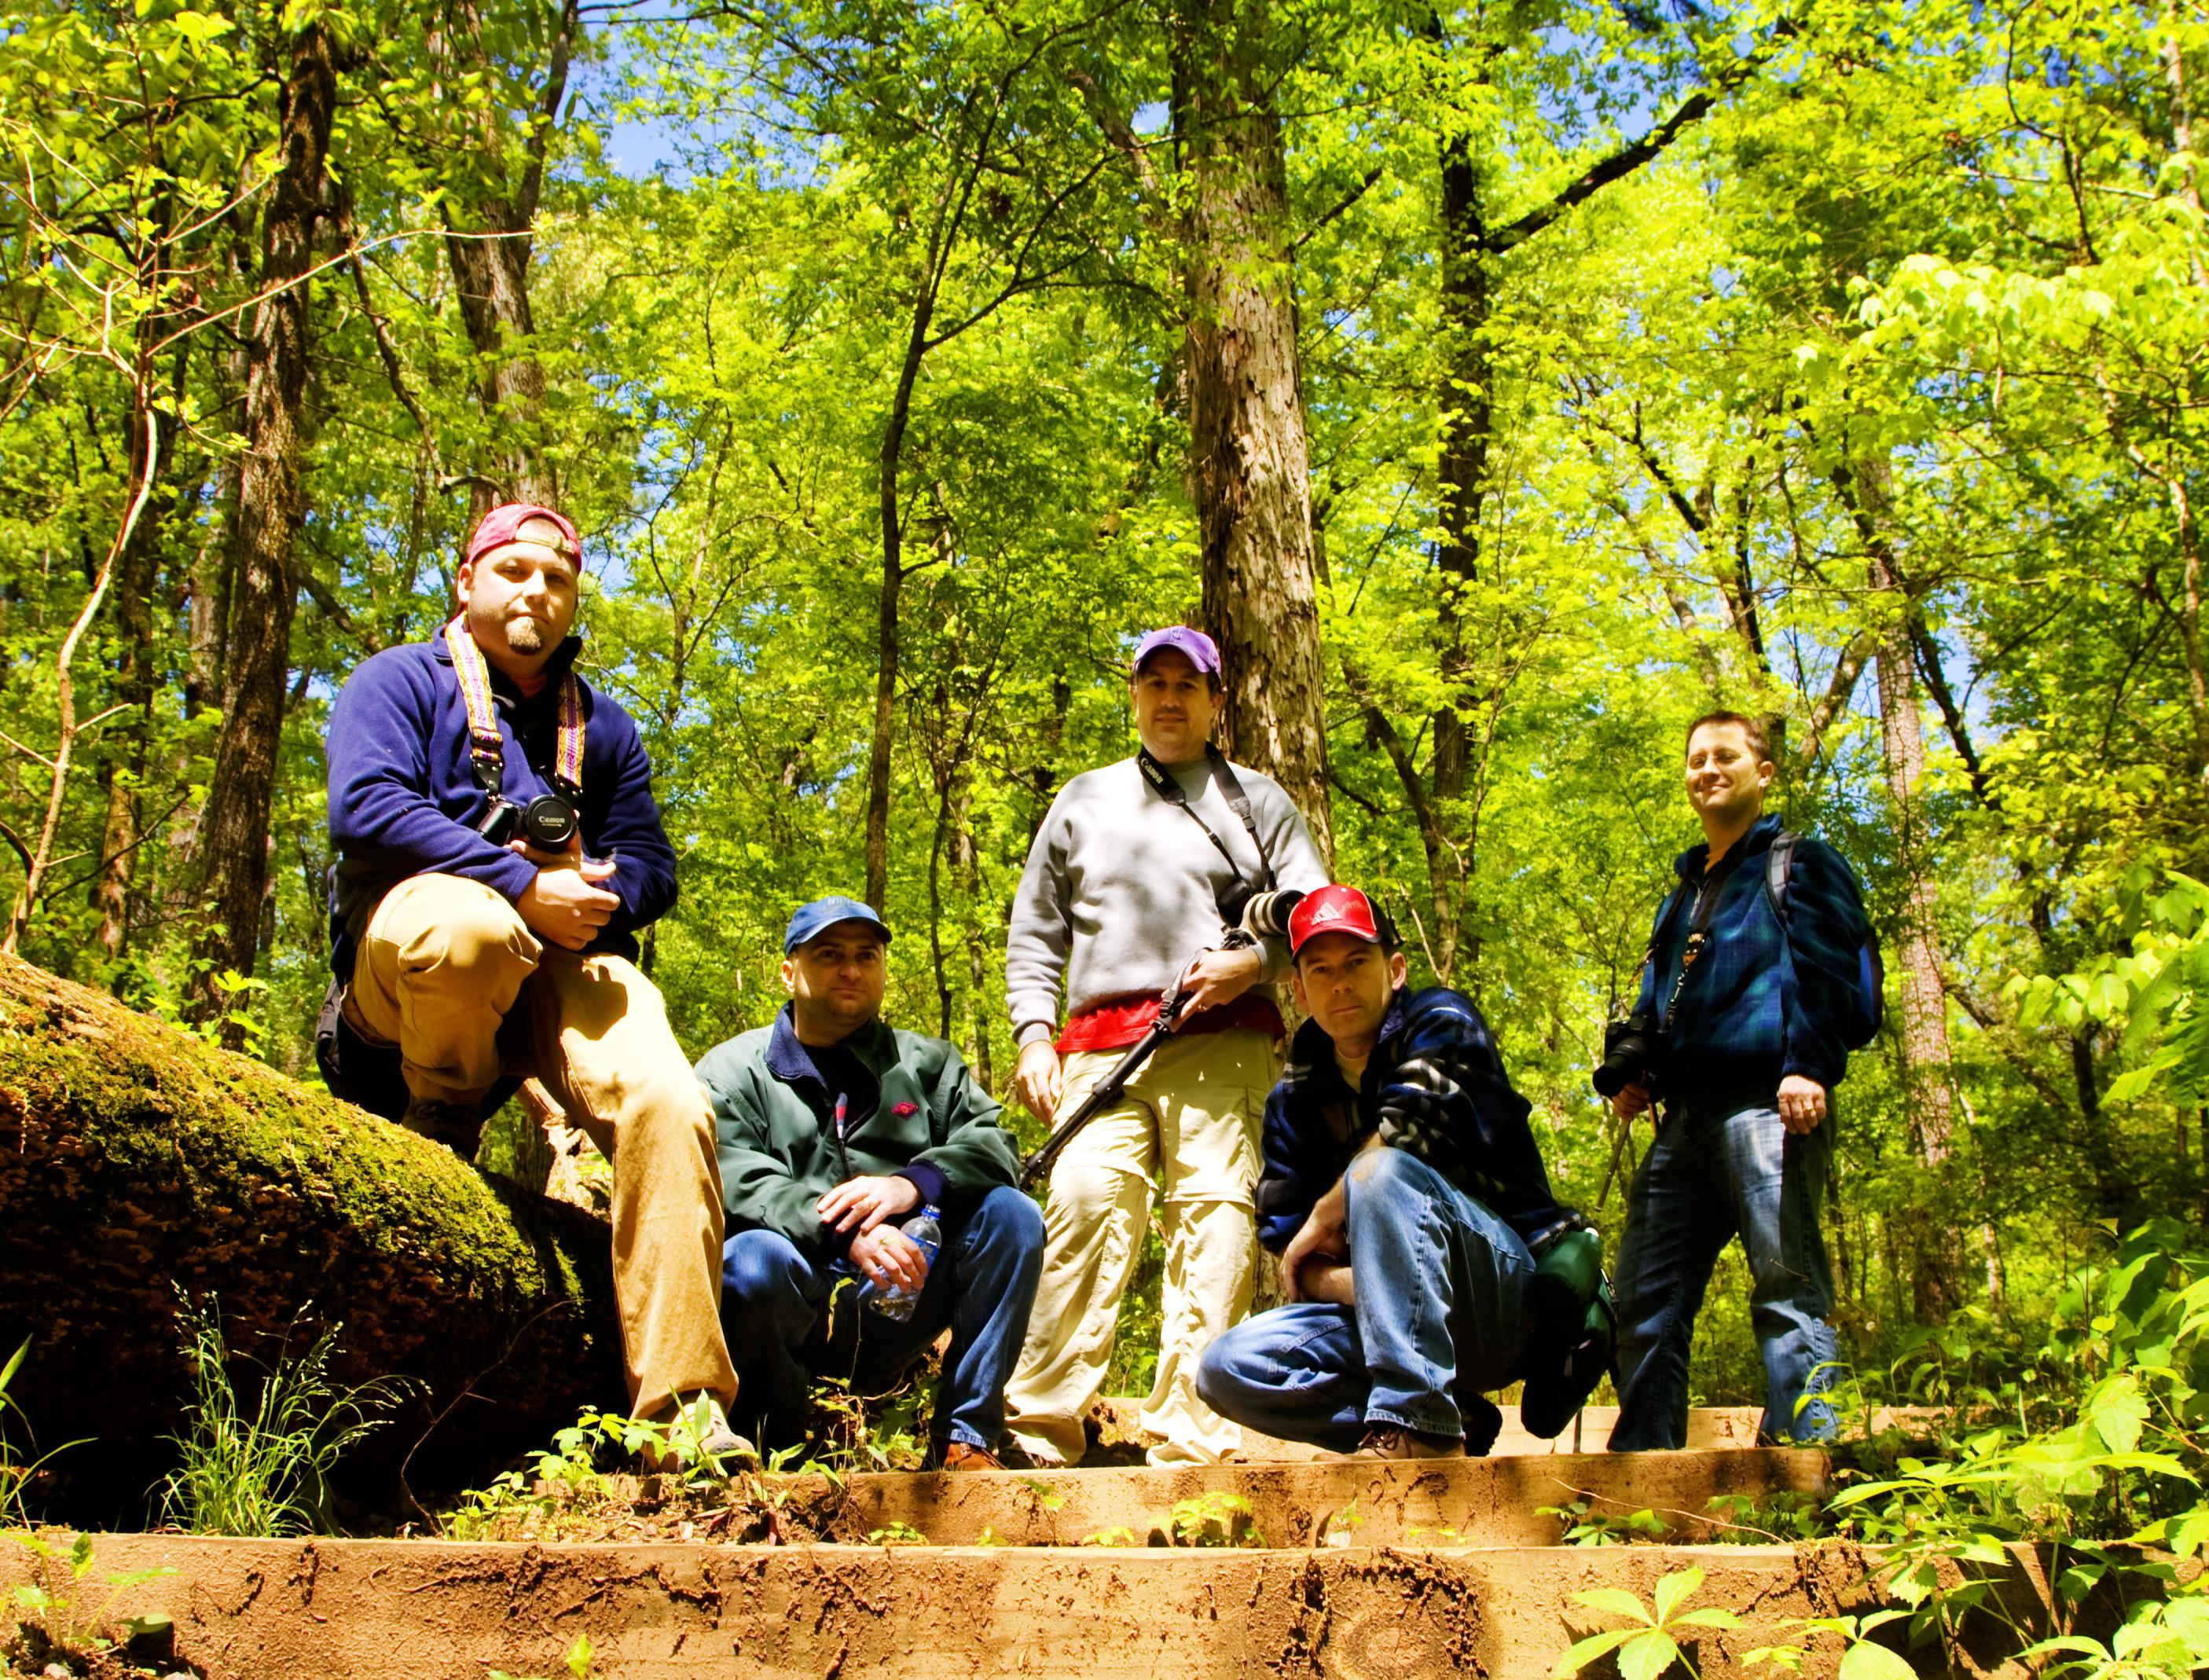
\includegraphics[width=\textwidth]{figures/data_5}
\end{subfigure}
\begin{subfigure}[b]{0.3\textwidth}
    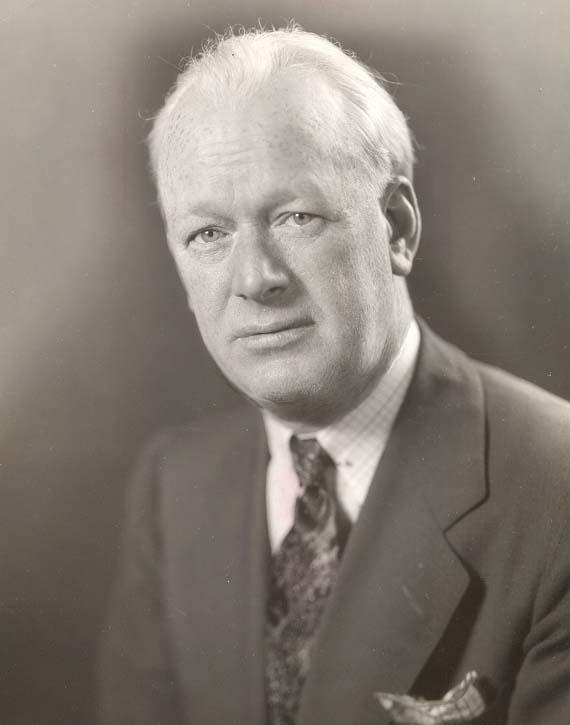
\includegraphics[width=\textwidth]{figures/data_6}
\end{subfigure}
\caption[常見人臉資料集中的圖片範例]{Wider Face 和 AFW 等常見人臉資料集中大部分是在正常光照下的圖片}
\label{fig:general_face}
\end{figure}

\begin{figure}[t]
\centering
\begin{subfigure}[b]{0.22\textwidth}
    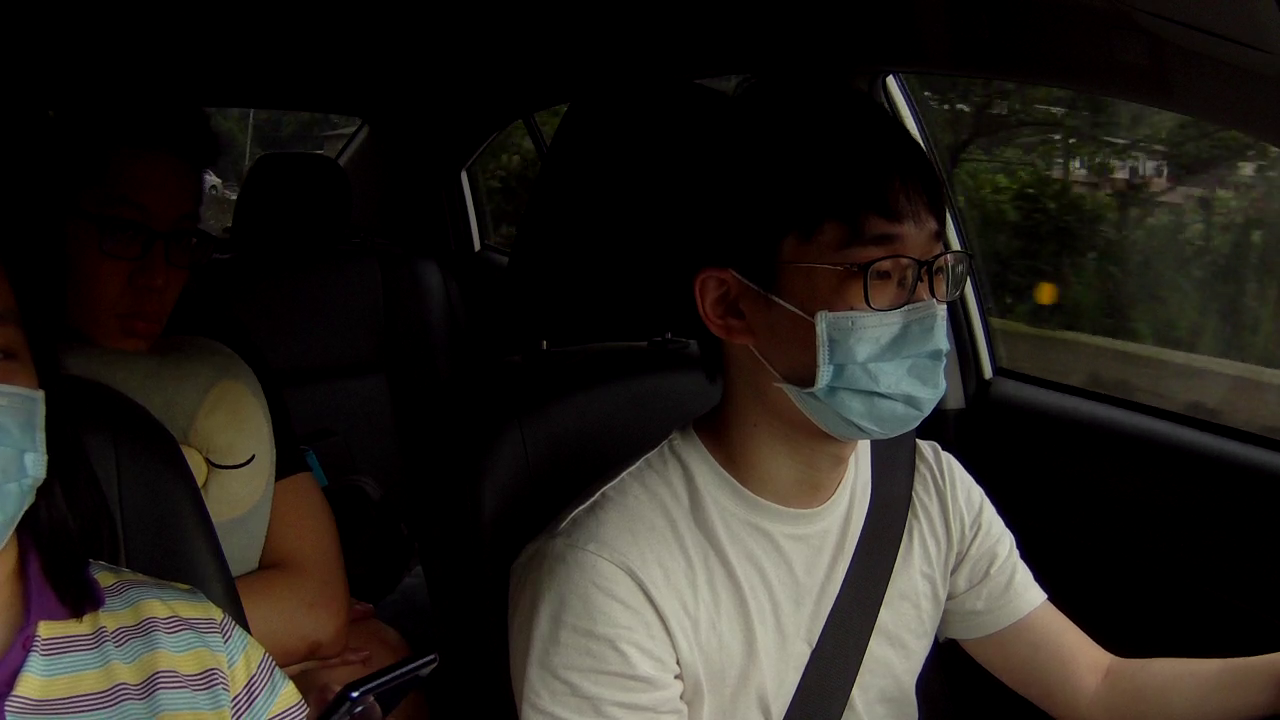
\includegraphics[width=\textwidth]{figures/car_1}
\end{subfigure}
\begin{subfigure}[b]{0.22\textwidth}
    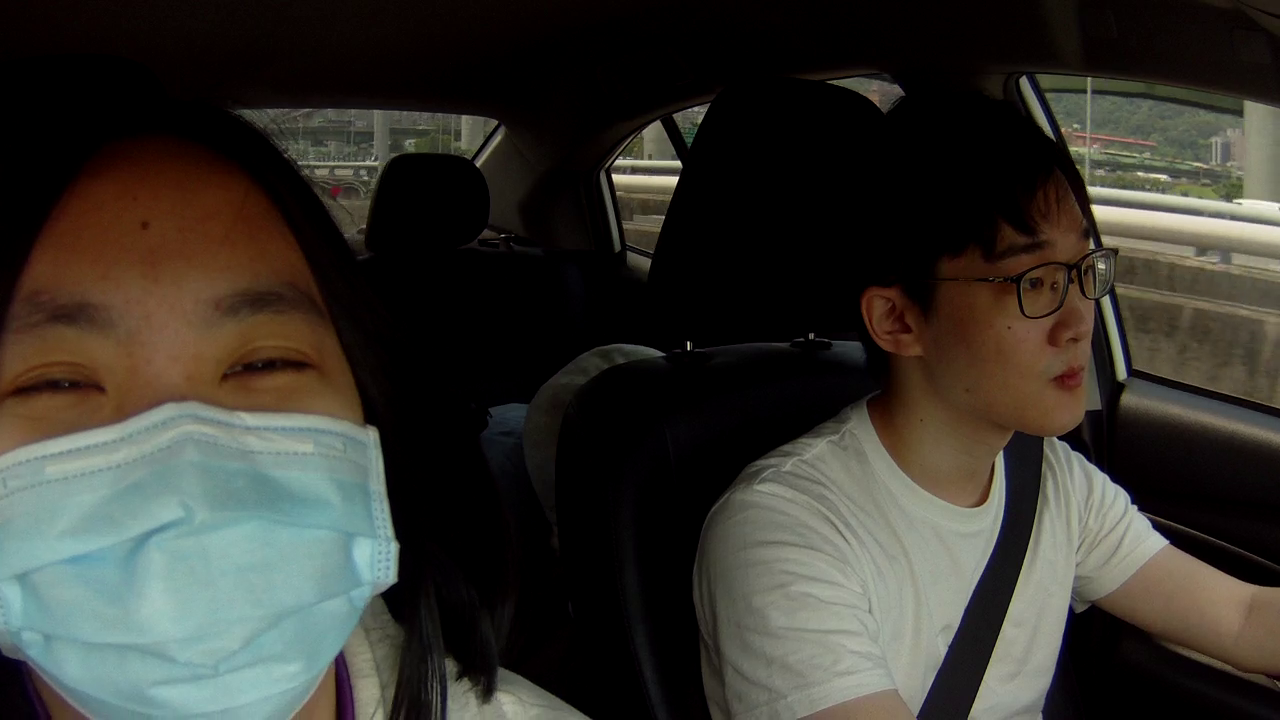
\includegraphics[width=\textwidth]{figures/car_2}
\end{subfigure}
\begin{subfigure}[b]{0.22\textwidth}
    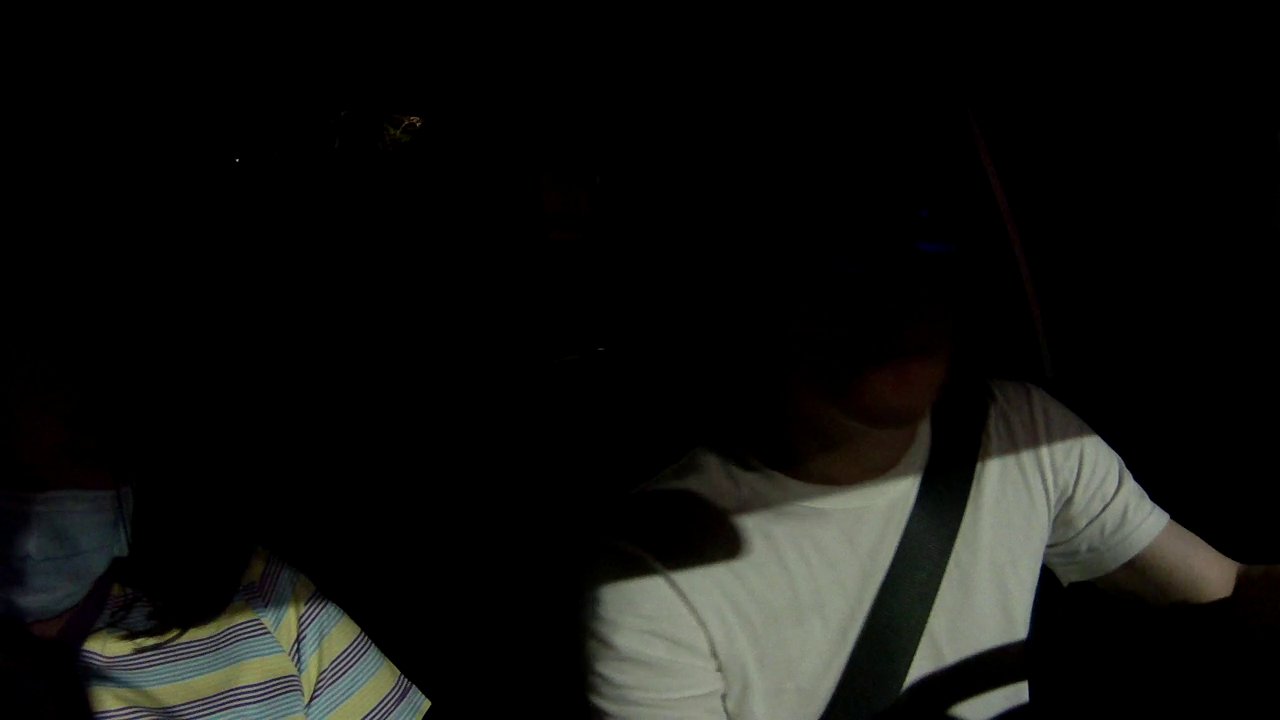
\includegraphics[width=\textwidth]{figures/car_3}
\end{subfigure}
\begin{subfigure}[b]{0.22\textwidth}
    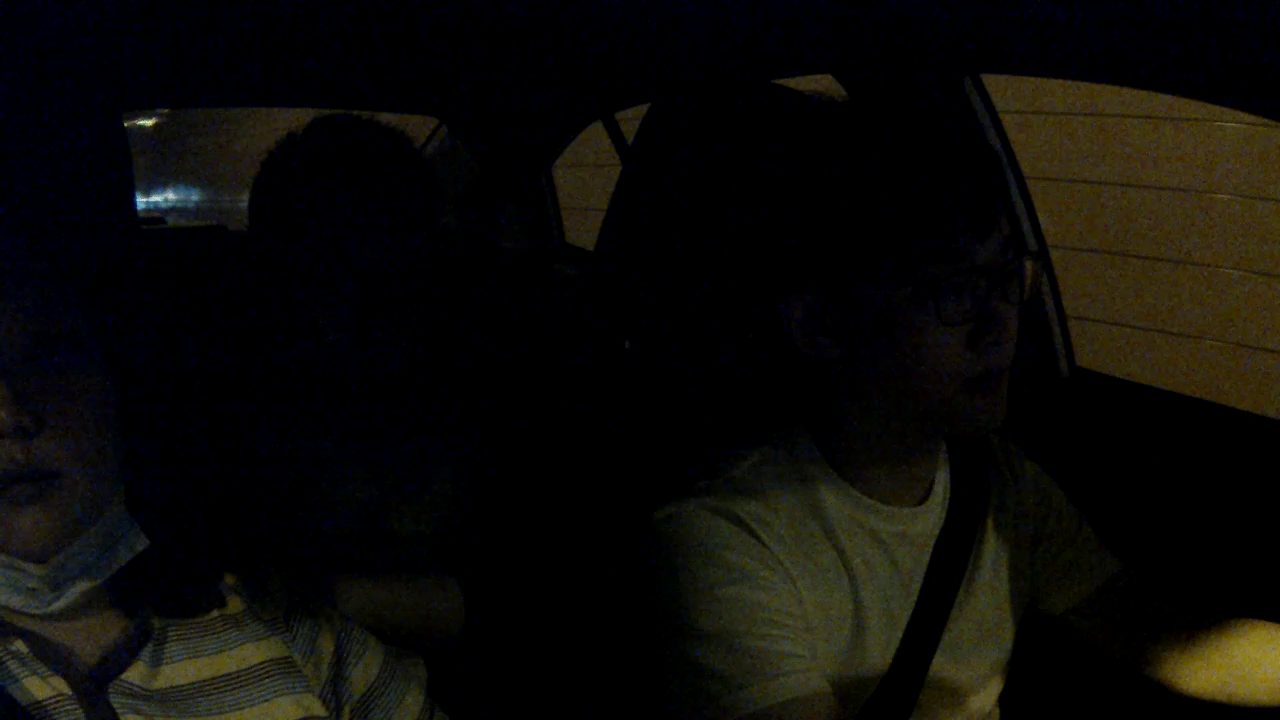
\includegraphics[width=\textwidth]{figures/car_4}
\end{subfigure}
\begin{subfigure}[b]{0.22\textwidth}
    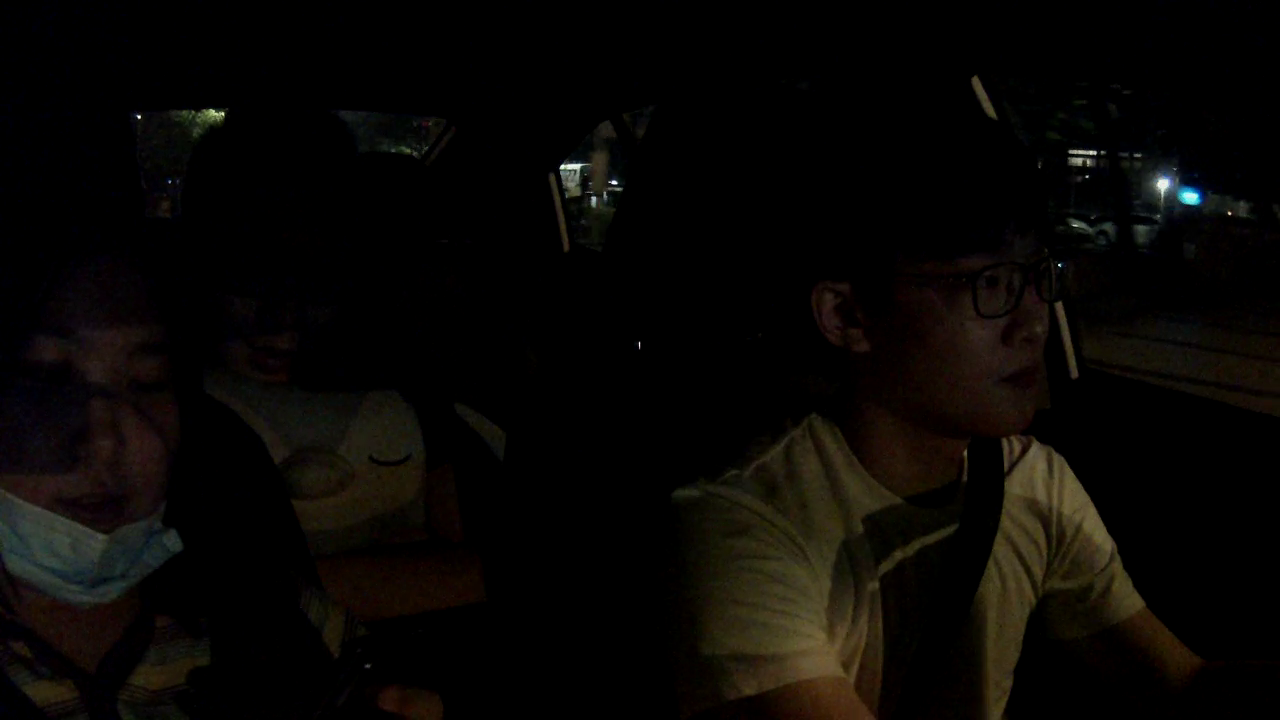
\includegraphics[width=\textwidth]{figures/car_5}
\end{subfigure}
\begin{subfigure}[b]{0.22\textwidth}
    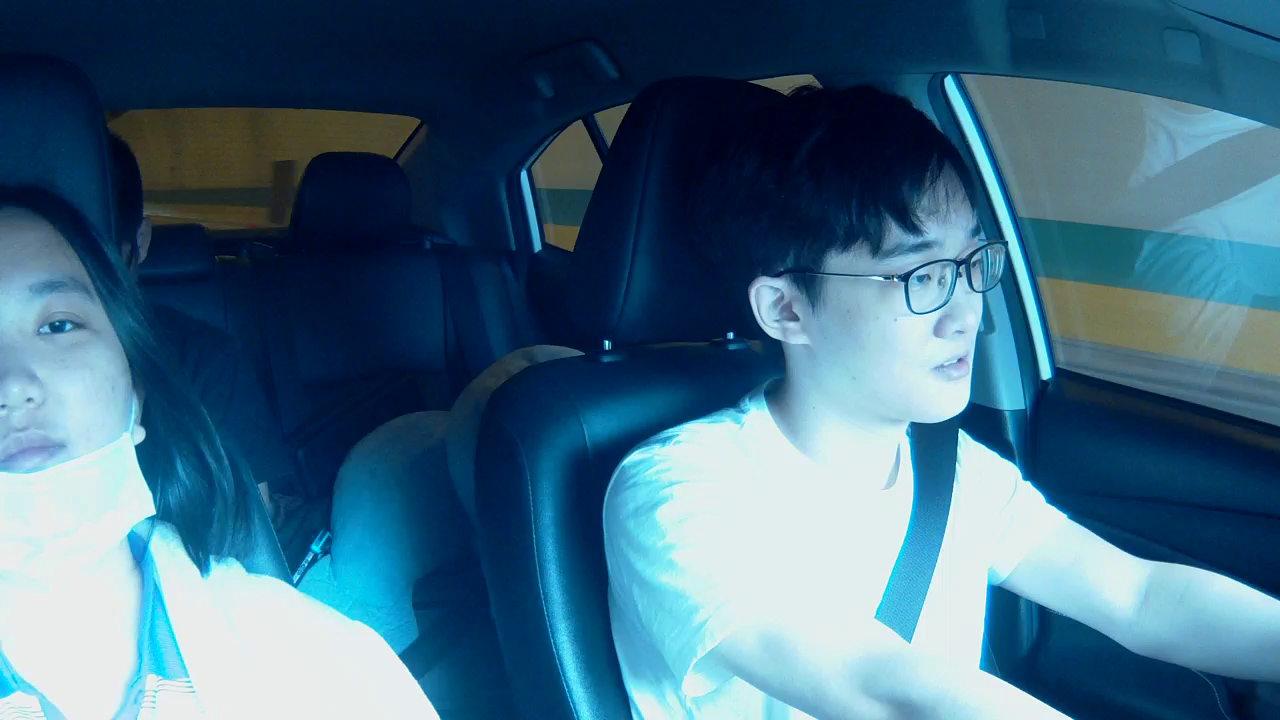
\includegraphics[width=\textwidth]{figures/car_6}
\end{subfigure}
\begin{subfigure}[b]{0.22\textwidth}
    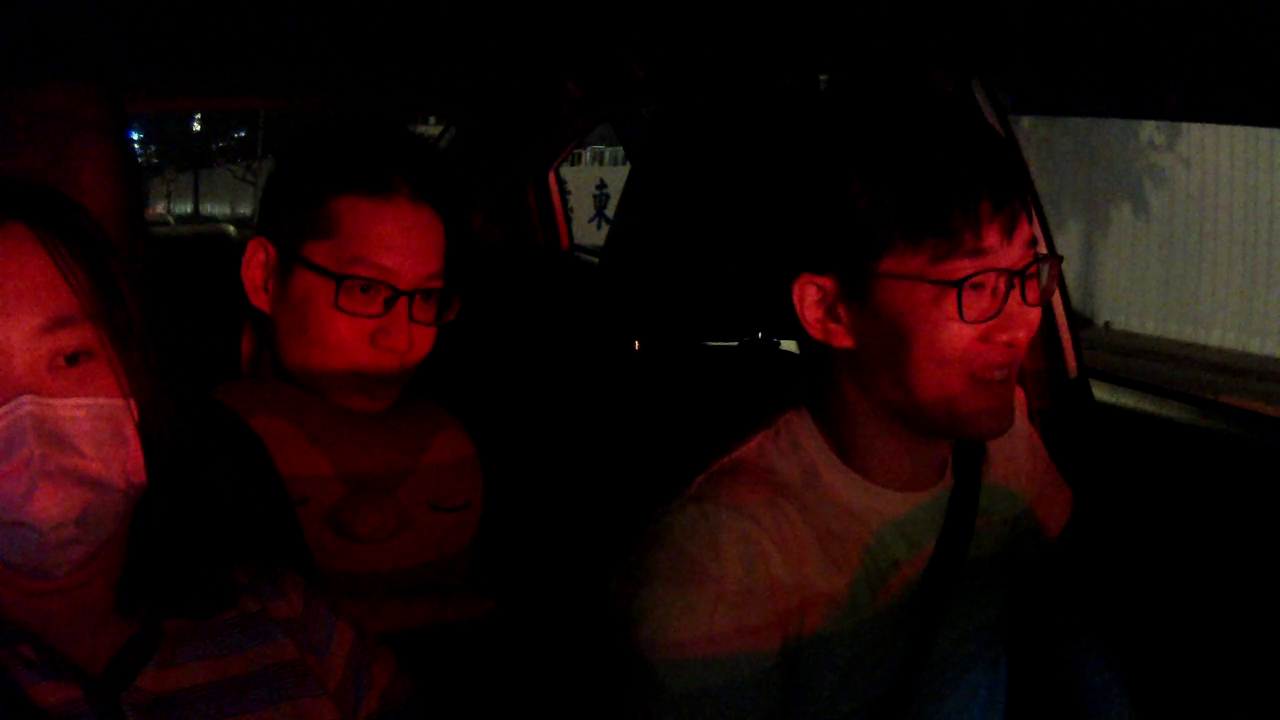
\includegraphics[width=\textwidth]{figures/car_7}
\end{subfigure}
\caption[車內影像範例]{車內影像包含各種光照下的圖片}
\label{fig:incar_face}
\end{figure}

為了解決這項問題,我們希望運用一些方法來消除光照對圖片造成的影響。過去也有不少電腦視覺的相關研究~\cite{cho2018face, kalaiselvi2013face, chen2018learning}在碰到光照問題時選擇對圖片進行增強處理,而我們也測試過增強部分低光照圖片確實能增加模型偵測出的人臉數量,因此我們原先也試過對圖片進行增強處理來解決問題。但我們馬上發現現行的增強方法大多專注於對低光照圖片的資訊恢復,應用在同時有極亮和極暗資料的訓練上測試結果就相對不佳 (如圖~\ref{train_compare})。
此時我們注意到其中一個用於影像增強的傳統演算法:直方圖均衡化,它雖然被歸類於影像增強,但在實作上它會重新分配圖中每個像素的數值使最後輸出結果的亮度在直方圖上分布均勻,本質上較接近將圖片的亮度進行正規化。這促使我們轉而思考如何將圖片的亮度進行正規化處理,使不同光照下的圖片在經過處理後能輸出相似的結果。

\begin{figure}[htb]
\centering
\begin{subfigure}[b]{0.3\textwidth}
    \centering
    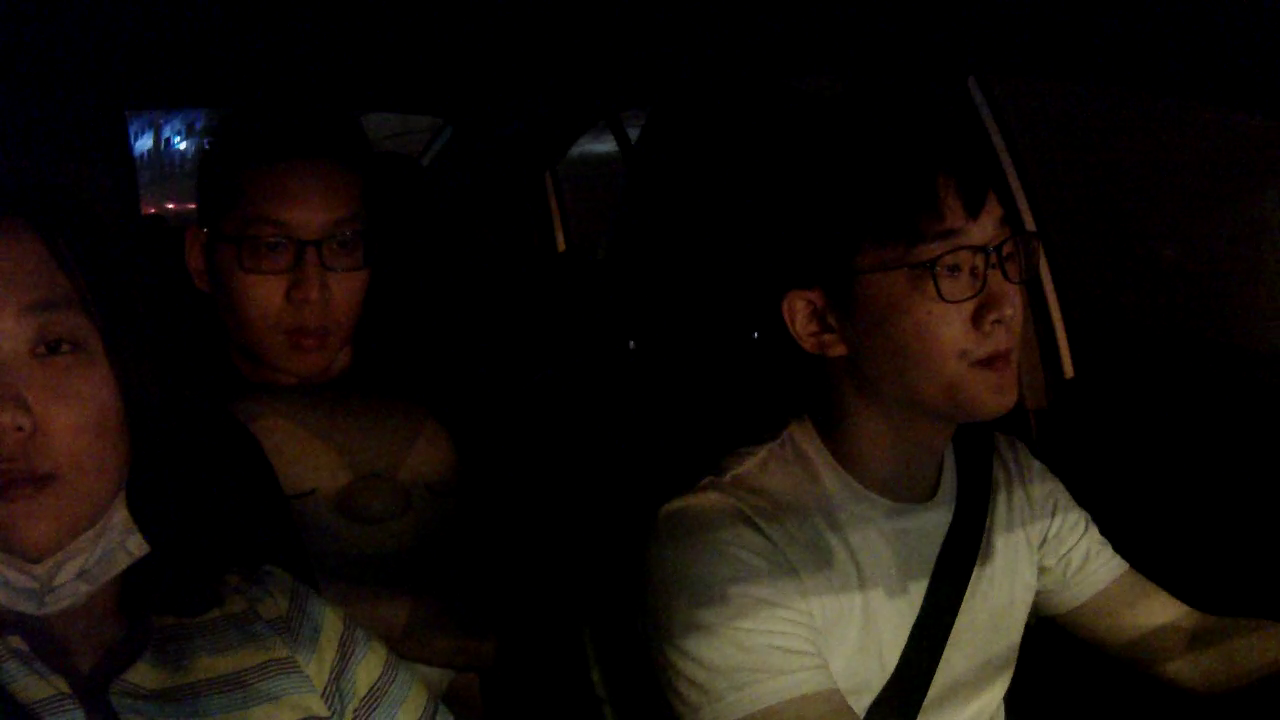
\includegraphics[width=\textwidth]{figures/ori_input}
    \caption{輸入圖片}
\end{subfigure}
\begin{subfigure}[b]{0.3\textwidth}
    \centering
    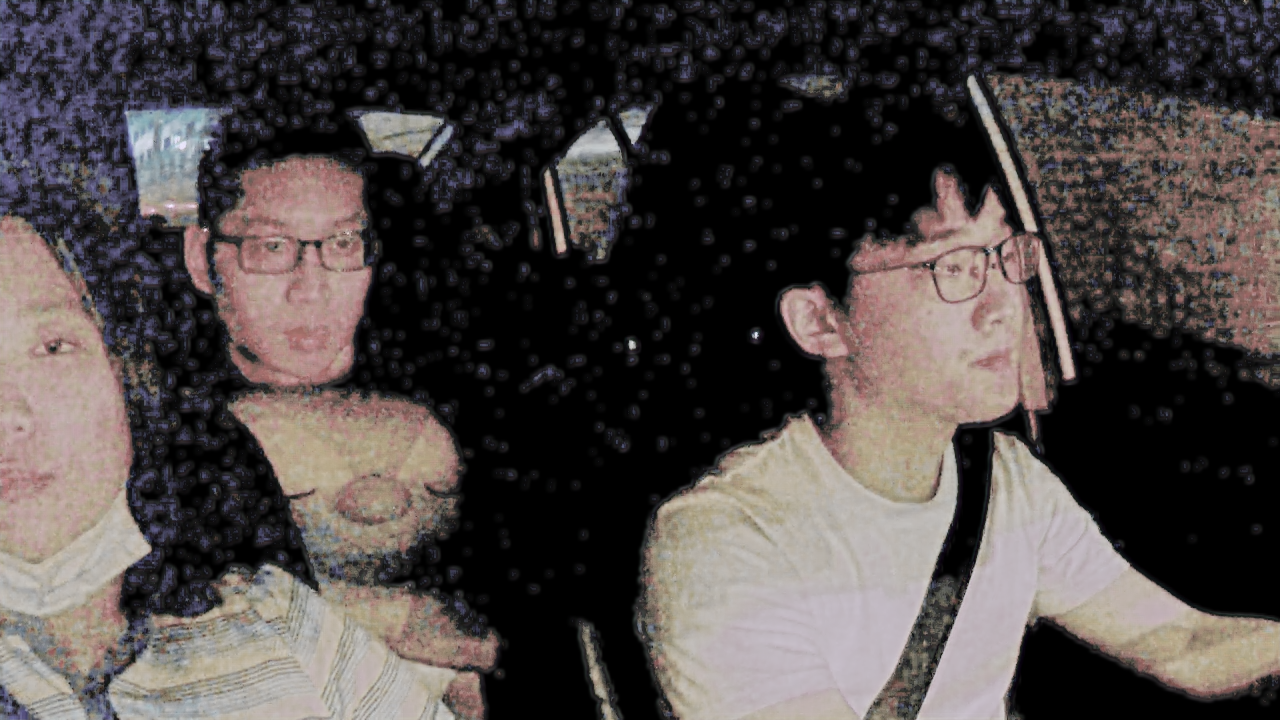
\includegraphics[width=\textwidth]{figures/dark_output}
    \caption{只以低光照圖片訓練的模型之輸出結果}
\end{subfigure}
\begin{subfigure}[b]{0.3\textwidth}
    \centering
    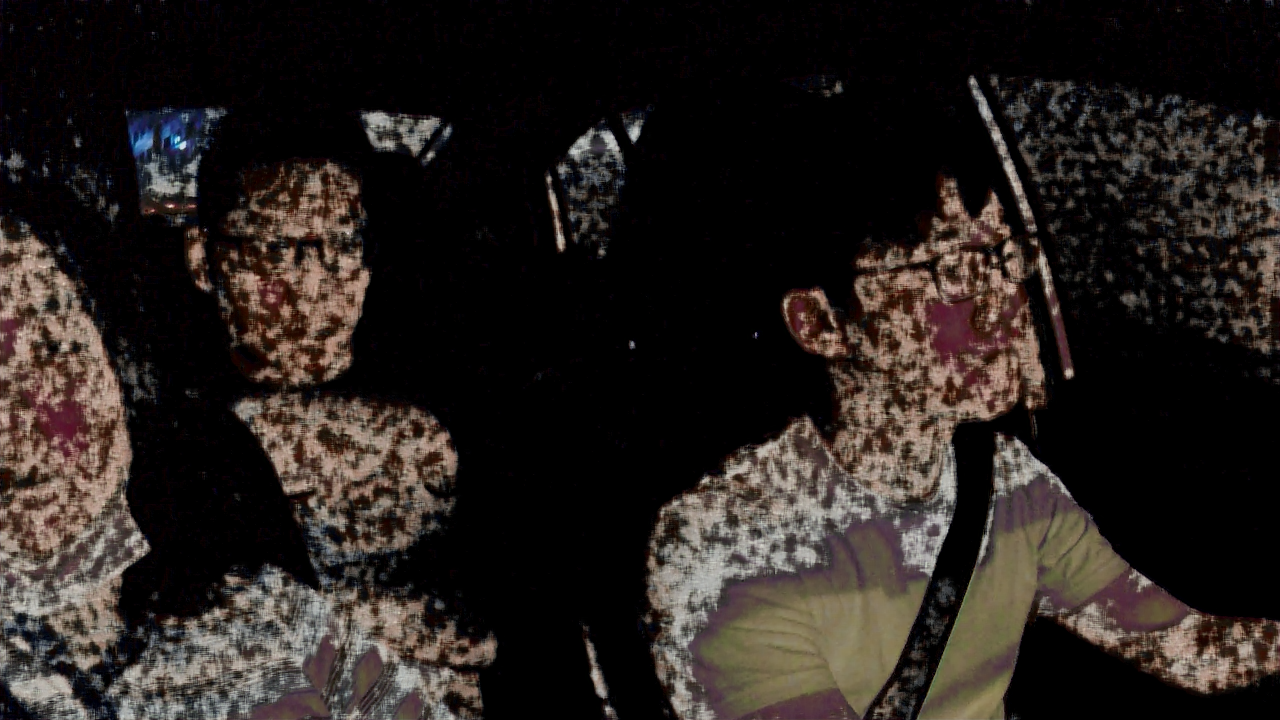
\includegraphics[width=\textwidth]{figures/both_output}
    \caption{同時以低 / 高光照圖片訓練的模型之輸出結果}
\end{subfigure}
\caption[訓練資料中含有高光照圖片與否之模型輸出結果比較]{增強模型原先應用於低亮度圖片的資訊恢復,而當我們在訓練資料中加入高光照的圖片後,訓練結果較為不佳}
\label{fig:train_compare}
\end{figure}

\section{方法}

我們的方法完整的測試流程如圖~\ref{fig:test_flow}所示。圖片在輸入模型之後會先經過正規器進行圖片的正規化處理,然後才會經過人臉偵測器算出偵測框結果。

我們完整的訓練流程則如圖~\ref{fig:train_flow}所示,分為兩個階段:預訓練和主要訓練。首先我們會先對正規器模型進行預訓練獲得初始權重,然後再將正規器和人臉偵測器接在一起進行主要訓練。以下我們分別就兩個訓練階段作詳細的說明。

\begin{figure}[htb]
\centering
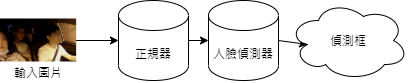
\includegraphics[width=0.8\textwidth]{figures/test_flow}
\caption[測試時從輸入圖片到獲得偵測結果的流程]{輸入圖片會先經過正規器 (Normalizer) 處理再經過人臉偵測器算出偵測框}
\label{fig:test_flow}
\end{figure}

\begin{figure}[htb]
\centering
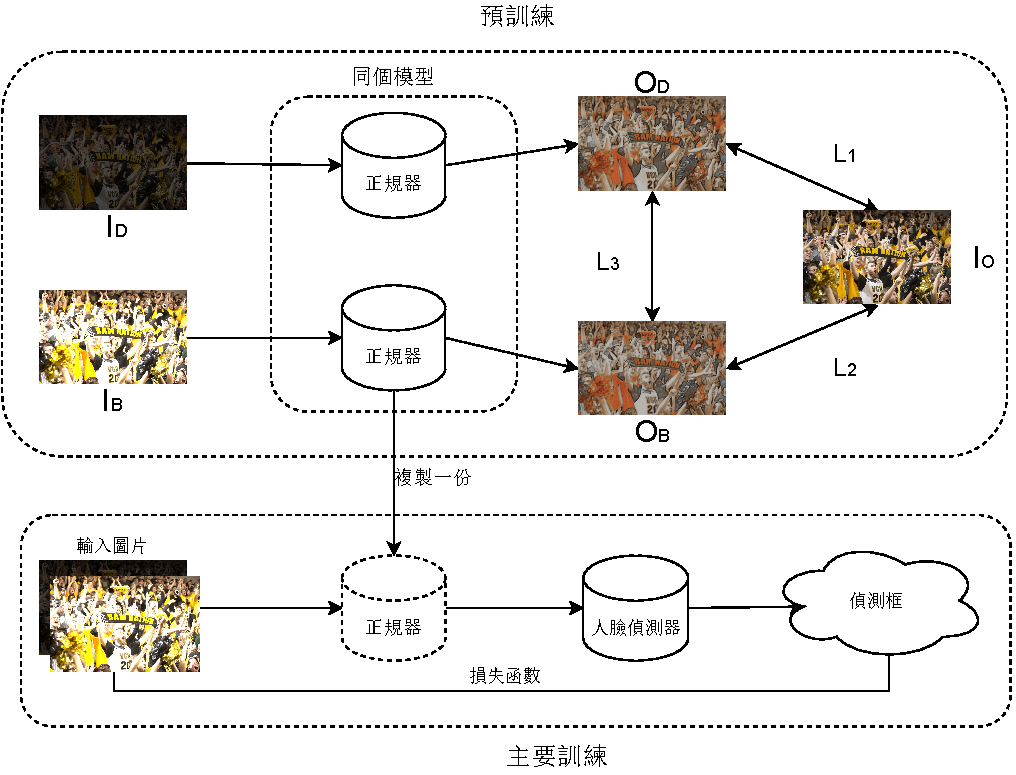
\includegraphics[width=1\textwidth]{figures/train_flow}
\caption[完整的訓練流程]{我們的訓練流程包含了預訓練和主要訓練}
\label{fig:train_flow}
\end{figure}

\subsection{預訓練}

在預訓練中,我們的目的是給正規器一個好的初始權重,以便在後續的主要訓練進行優化。

對於正規器的訓練,我們原先的想法是輸入一張過高或過低光照的圖和一張作為基準真相 (Ground Truth) 同一場景下正常光照的圖,對模型進行監督式學習 (如圖~\ref{fig:original_pretrain}),試圖把輸入圖片的光照調整為正常值。
但由於在主要訓練階段我們會將正規器和人臉偵測器接在一起做端對端訓練,為了不要讓整體模型的深度太深,我們會選擇架構較簡單、參數較少的模型作為正規器的架構。而這樣的選擇帶來的一個問題便是正規器的模型較弱,直接作監督式學習的結果不佳。
為了能順利訓練正規器,我們設計了一套三圖一組的訓練架構 (如圖~\ref{fig:triple_setting})。以下我們分別就這套訓練架構中的損失函數、資料和所使用的模型進行說明。

\begin{figure}[htb]
\centering
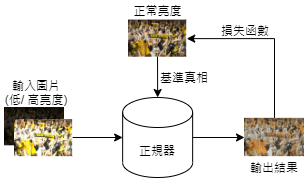
\includegraphics[width=1\textwidth]{figures/original_pretrain}
\caption[預訓練時我們嘗試過的架構]{原先我們嘗試輸入一張過高或過低光照的圖和一張作為基準真相同一場景下正常光照的圖,對模型進行監督式學習}
\label{fig:original_pretrain}
\end{figure}

\begin{figure}[htb]
\centering
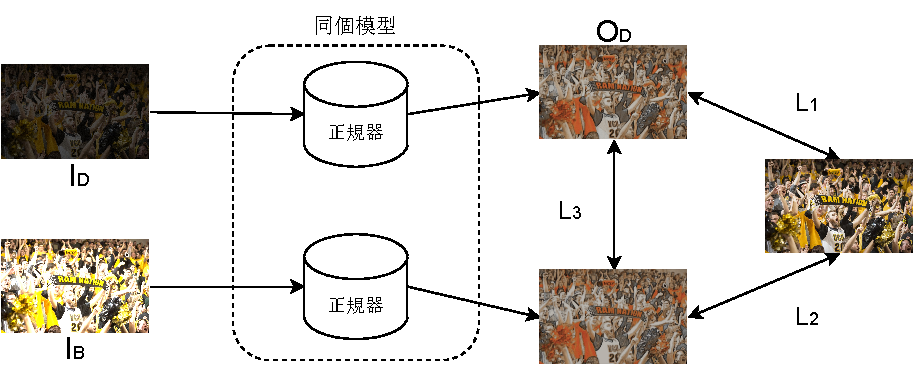
\includegraphics[width=1\textwidth]{figures/triple_setting}
\caption[預訓練時所採用的架構]{我們在預訓練時使用三圖一組架構來訓練正規器}
\label{fig:triple_setting}
\end{figure}

\subsubsection{損失函數}

我們希望設計出的損失函數能使在不同光照下的圖片被正規化成相似的結果,以便進行後續的人臉偵測。為了達成這個目標,我們對同一場景在三個不同光照條件下的圖片進行比較。這個想法首先來自於前述的監督式學習。我們判斷以正常光照下的圖做為參考直接作監督式學習對模型而言太過困難,其理由包括了至少以下兩點:

1. 為了降低整體模型的深度,我們選擇的正規器模型架構較簡單、參數較少,是個比較弱的模型。

2. 我們用來作參考的圖雖然都是在正常光照下,但其實不同圖片間的亮度標準差不小,監督式學習難以判斷要將輸入圖片調整成什麼樣子。

為此我們決定將問題簡單化,只要求不同光照下的輸入圖片在經過處理後,圖片的亮度能收斂到某幾個值,並不要求輸出的圖片看起來應該要和同一場景在正常光照下的圖片相似。但如此一來,我們就不能直接作監督式學習,而需要用較迂迴的方式訓練模型。為此我們設計了三圖一組的架構,這個架構受到了 FaceNet~\cite{schroff2015facenet} 的啟發,他們在論文中設計的損失函數會透過比較三個點之間的距離來修改參數權重。在概念上我們的損失函數定義如下:
$$L_{Total} = \alpha L_{Content} + L_{Light}$$
其中 $L_{Light}$ 的用意是使不同光照下的輸入在經過處理後能有盡量一致的長相,但如果只使用 $L_{Light}$ 的話,我們可能會訓練出一個不顧輸入圖片長相一律輸出同樣結果的模型。因此為了使學出來的模型能兼顧保留場景原本樣貌和消除光線影響,我們加入了 $L_{Content}$ 以保留場景中的資訊。$\alpha$ 在這裡作為一個調整兩個損失函數間取捨的超參數,當 $\alpha$ 越小,代表我們越傾向讓輸入圖片經過處理的結果一致,此時我們獲得的結果圖片會越來越模糊;而當$\alpha$越大,代表我們越強調要保留場景中的資訊,此時模型的訓練模式便會越來越接近原本的監督式學習,因乏適 (Underfitting) 而使結果圖片出現雜訊 (如圖)。

我們使用三張一組的圖片來實作上述損失函數的細節,每一組圖片包含了同一場景在曝光正常、曝光不足、曝光過度這三種情況下的圖片,以下稱 $I_O$、$I_D$、$I_B$。我們讓 $I_D$ 和 $I_B$ 在經過正規器後輸出的兩個結果 (以下稱 $O_D$ 和 $O_B$) 算出兩張圖間的損失函數 $L_3$。為了使兩張圖之間的距離越小越好,我們在這裡使用了 $L2$ 損失函數。同時為了不使這兩個結果和原圖相差過大,我們讓 $O_D$ 和 $O_B$ 分別和 $I_O$ 算出兩個損失函數 $L_1$ 和 $L_2$,在這裡我們同樣使用了 $L2$ 損失函數。這三個損失函數和我們在前面定義的損失函數關係如下:
$$L_{Light} = L_3 = \mathcal{L}^{\ell_2}(O_D, O_B)$$
$$L_{Content} = L_1 + L_2 = \mathcal{L}^{\ell_2}(O_D, I_O) + \mathcal{L}^{\ell_2}(O_B, I_O)$$
於是完整的損失函數定義如下:
$$L_{Total} = \alpha (L_1 + L_2) + L_3$$

\subsubsection{資料}

由於利用真實資料會有收集上的困難,也較難保證場景中的內容物不變,我們在此架構中所使用三張一組的資料是透過演算法將原始圖片做調整,模擬出曝光不足和曝光過度這兩個情境下的圖片 (示意如圖~\ref{fig:same_triple})。以下分別說明兩種情境下的調整:

\begin{figure}[htb]
\centering
\begin{subfigure}[b]{0.3\textwidth}
    \centering
    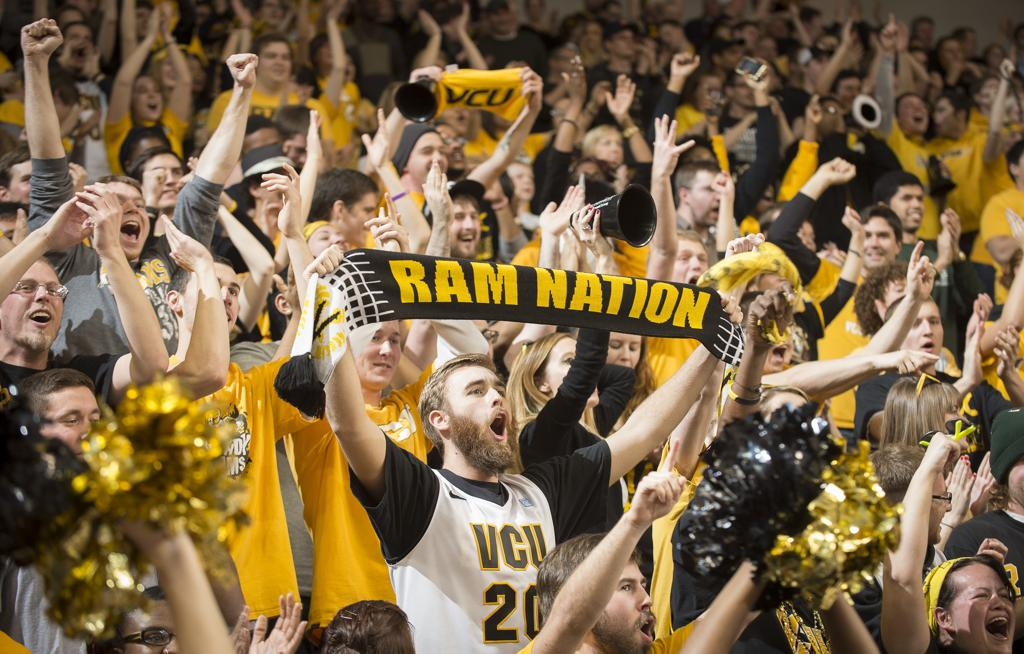
\includegraphics[width=\textwidth]{figures/same_original}
    \caption{原始圖片}
\end{subfigure}
\begin{subfigure}[b]{0.3\textwidth}
    \centering
    
\includegraphics[width=\textwidth]{figures/same_dark}
    \caption{曝光不足模擬後}
\end{subfigure}
\begin{subfigure}[b]{0.3\textwidth}
    \centering
    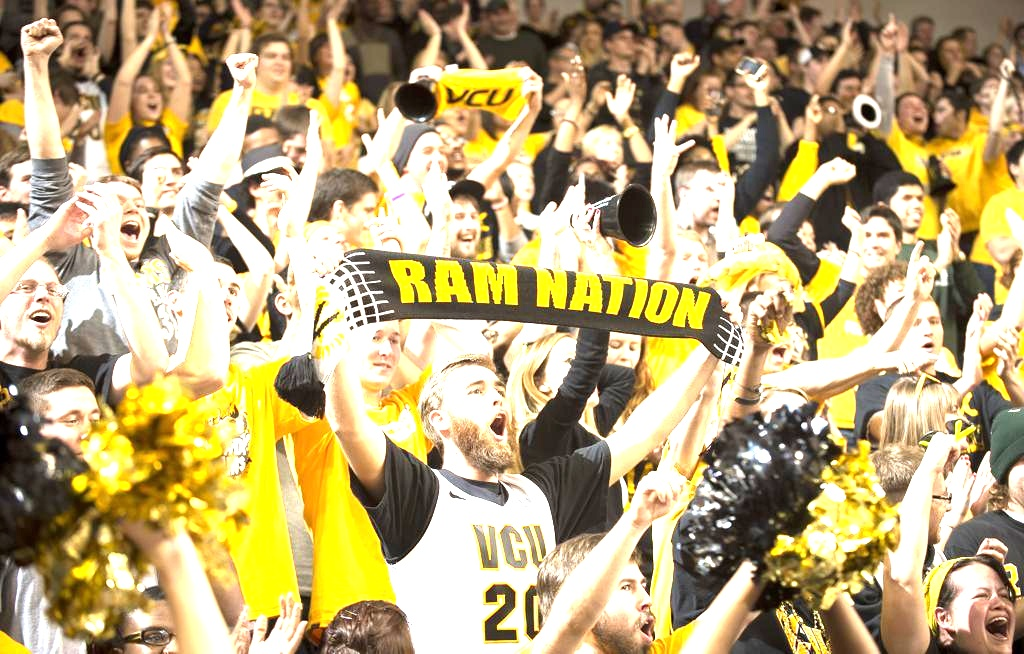
\includegraphics[width=\textwidth]{figures/same_bright}
    \caption{曝光過度模擬後}
\end{subfigure}
\caption[不同光照模擬下的同一場景]{同一場景經過不同光照模擬後的示意圖}
\label{fig:same_triple}
\end{figure}

\textbf{模擬曝光不足}

1. 對每個像素 $P = (r, g, b)$ 調整亮度至 $l\%$ ($l < 1$)
\begin{align*}
(h, s, v) &= \text{RgbToHsv}(r, g, b) \\
v' &= (\frac{v^{2.2}}{255} \times l\%)^{\frac{1}{2.2}} \times 255 \\
P' &= \text{HsvToRgb}(h, s, v')
\end{align*}
2. 對每個調暗過後的像素 P' 增加高斯雜訊
\begin{align*}
P'' &= P' + n\\
\text{where } n &\sim N(0, \sigma^2)
\end{align*}

\textbf{模擬曝光過度}

對每個像素 $P = (r, g, b)$ 調整亮度至 $l\%$ ($l > 1$)
\begin{align*}
(h, s, v) &= \text{RgbToHsv}(r, g, b) \\
v' &= (\frac{v^{2.2}}{255} \times l\%)^{\frac{1}{2.2}} \times 255 \\
P' &= \text{HsvToRgb}(h, s, v')
\end{align*}

\subsubsection{所使用的模型}

在此架構中我們使用了 MSR-net~\cite{shen2017msr} 來作為正規器的架構。它是一個能夠對低亮度圖片做影像增強的模型,能夠對圖片作局部亮度的調整。在架構上它的設計基於卷積神經網路,能夠接受不同大小的輸入資料;而在尺寸上它和其他影像增強的模型相比較為輕量,方便我們在進行預訓練後將其和偵測器接在一起作端對端的訓練優化。

在預訓練中,我們使用三圖一組的架構搭配特別設計的損失函數與用演算法模擬的資料對模型進行訓練。在預訓練結束後,我們就能獲得一個能夠消除光線對圖片影響的正規器。

\subsection{主要訓練}

在主要訓練中,我們將正規器和人臉偵測器接在一起做端對端訓練。
我們的目標是讓來自不同光線照射下的圖片在經過正規化處理後能夠有更多人臉成功被偵測出來。為了模擬不同光線照射下的情境,我們使用了上一節提到的演算法對訓練用的資料做了不同光線照射下的模擬,讓輸入資料包含曝光不足和曝光過度情境下的圖片。

而在模型架構上,我們選擇了 FaceBoxes~\cite{zhang2017faceboxes} 作為主要訓練中人臉偵測器的架構。它是一個基於卷積神經網路的人臉偵測器,透過對卷積層作優化來達到高效率高精確率人臉偵測。由於長遠來說我們希望能夠在車內進行高效率的人臉偵測,因此它對我們來說是個很好的選擇。

主要訓練結束後,我們獲得最終的人臉偵測器模型。